\documentclass[11pt, a4paper]{article}

\usepackage{amsmath}
\usepackage{amssymb}

% fonts
\usepackage{xeCJK}
\setCJKmainfont[BoldFont=SimHei]{SimSun}
\setCJKfamilyfont{hei}{SimHei}
\setCJKfamilyfont{kai}{KaiTi}
\setCJKfamilyfont{fang}{FangSong}
\newcommand{\hei}{\CJKfamily{hei}}
\newcommand{\kai}{\CJKfamily{kai}}
\newcommand{\fang}{\CJKfamily{fang}}

% style
\usepackage[top=2.54cm, bottom=2.54cm, left=3.18cm, right=3.18cm]{geometry}
\linespread{1.5}
\usepackage{indentfirst}
\parindent 2em
\punctstyle{quanjiao}
\renewcommand{\today}{\number\year 年 \number\month 月 \number\day 日}

% figures and tables
\usepackage{graphicx}
\usepackage[font={bf, footnotesize}, textfont=md]{caption}
\makeatletter
    \newcommand\fcaption{\def\@captype{figure}\caption}
    \newcommand\tcaption{\def\@captype{table}\caption}
\makeatother
\usepackage{booktabs}
\renewcommand\figurename{图}
\renewcommand\tablename{表}
\newcommand{\fref}[1]{\textbf{图\ref{#1}}}
\newcommand{\tref}[1]{\textbf{表\ref{#1}}}
\newcommand{\tabincell}[2]{\begin{tabular}{@{}#1@{}}#2\end{tabular}} % multiply lines in one grid

\usepackage{listings}
\lstset{basicstyle=\ttfamily}

\usepackage{xcolor}
\renewcommand{\r}{\color{red}}

\usepackage{url}

% tikz
\usepackage{tikz}
\usetikzlibrary{shapes.geometric, arrows}

\tikzstyle{actor} = [rectangle, rounded corners, minimum width=3cm, minimum height=1cm, text centered, draw=black, fill=red!30]
\tikzstyle{module} = [rectangle, minimum width=3cm, minimum height=1cm, text centered, draw=black, fill=orange!30]
\tikzstyle{arrow} = [thick,<->,>=stealth]

% syntax
\usepackage{syntax}

% start of document
\title{\textbf{\texttt{mydb}数据库设计报告}}
\author{\kai 朱俸民\quad 2012011894
\and \kai 温和\quad 2013011407}
\date{\kai \today}

\begin{document}

\maketitle

\section{功能介绍}

\texttt{mydb}是一个简单的面向单用户、单线程的关系数据库管理系统,支持增、查、删、改四项基本数据库查询功能,通过SQL的一个子集实现数据库与用户的交互。除了支持基本的增、查、删、改功能外,\texttt{mydb}具有如下扩展功能:

\begin{enumerate}
    \item 索引:使用\texttt{std::multimap}实现,支持对任意列建立索引加速约束检查;
    \item 域完整性约束:支持\texttt{CHECK}语句的创建,并在更新数据库时进行约束检查;
    \item 外键约束:支持\texttt{FOREIGN KEY}的创建,并在更新数据库时进行约束检查;
    \item 模糊查询:支持使用\texttt{LIKE}语句进行模糊匹配;
    \item 支持多表连接查询,包括三个表以上的连接;
    \item 聚集查询:支持将\texttt{SUM},\texttt{AVG},\texttt{MAX},\texttt{MIN}这四个函数应用于表中的某些列;
    \item 分组聚集查询:支持查询时的\texttt{GROUP BY}语句,可以处理聚集查询与分组聚集查询并存的查询;
    \item 完整的建表属性约束:建表时除了允许\texttt{NOT NULL},\texttt{PRIMARY KEY},\texttt{FOREIGN KEY}与\texttt{CHECK}约束外,还可以设置\texttt{UNIQUE},\texttt{AUTO\_INCREMENT}与\texttt{DEFAULT}约束;
    \item 在查询时,支持\texttt{BETWEEN}和\texttt{IN}操作符;
    \item 远程连接:允许远程开启\texttt{mydb}服务端后,本地用\texttt{mydb}客户端进行连接,通过SQL语句交互的方式进行数据库操作;
    \item 采用\texttt{MySQL}风格打印查询结果,易于用户查看。
\end{enumerate}

\section{系统架构}

\texttt{mydb}的顶层设计架构如\fref{arch}所示。

\begin{center}
    \begin{tikzpicture}[node distance=2cm]
        \node (user) [actor] {用户};
        \node (engine) [module, below of=user] {用户交互模块};
        \node (parse) [module, below of=engine] {SQL解析模块};
        \node (exe) [module, below of=parse] {SQL执行模块};
        \node (sys) [module, below of=exe, xshift=2cm] {系统管理模块};
        \node (record) [module, below of=exe, xshift=-2cm] {记录管理模块};
        \node (table) [actor, below of=sys, xshift=-2cm] {系统表};
        \node (config) [actor, below of=sys, xshift=2cm] {配置文件};
        \node (fs) [actor, below of=record, xshift=-2cm] {页式文件系统};
 
        \draw [arrow] (user) -- (engine);
        \draw [arrow] (engine) -- (parse);
        \draw [arrow] (parse) -- (exe);
        \draw [arrow] (exe) -- (sys);
        \draw [arrow] (exe) -- (record);
        \draw [arrow] (sys) -- (table);
        \draw [arrow] (sys) -- (config);
        \draw [arrow] (record) -- (fs);
    \end{tikzpicture}
    \fcaption{系统架构}\label{arch}
\end{center}

\section{模块设计}

接下来我们详细介绍各模块的设计与实现方法。

\subsection{记录管理模块}

在数据存储上,某个数据库 (database) 的某一张表 (table) 对应于与数据库同名的目录下与表同名的一个文件。在访问该表时,调用提供的页式文件系统进行文件读写,其中,每页大小均为8KB。我们定义,该文件对应的各页中,第1页 (即编号为0的页) 存储与记录 (record) 相关的元数据,其数据格式如\tref{record:metadata}所示。

\begin{center}
    \tcaption{元数据记录格式}\label{record:metadata}
    \begin{tabular}{ll}
        \toprule
        偏移量 (字节) & 记录信息 \\
        \midrule
        0 & 每条记录长度 \\
        4 & 记录总个数 \\
        8 & 最后一条记录的ID (rid) \\
        12 & 最后一页的编号 (pid) \\
        1024 & 空闲页位图 \\
        \bottomrule
    \end{tabular}
\end{center}

其中,空闲页位图大小总计7K,用1表示空闲,0表示占用。之后的每一页,均用于存储各条记录的数据。这些页的前32字节为空闲位图,记录该页哪些位置处可以用来存放新的记录,共计256位,分别对应该页的每32个字节 (称为一个\textbf{字}) 是否可用。因此,所有的记录必须按一个字对齐。对于具有$n$列的一条记录,其数据格式如\tref{record:record}所示。

\begin{center}
    \tcaption{记录数据格式}\label{record:record}
    \begin{tabular}{ll}
        \toprule
        偏移量 (字节) & 记录信息 \\
        \midrule
        0 & 记录ID (rid)  \\
        4 & 各字段是否为空的位图 \\
        $4+n$ & 记录的数据 \\
        \bottomrule
    \end{tabular}
\end{center}

对于记录的数据,我们按照列的顺序依次存储,我们支持如\tref{record:types}所示的数据类型。

\begin{center}
    \tcaption{支持的数据类型}\label{record:types}
    \begin{tabular}{lll}
        \toprule
        类型 & 映射的C++类型 & 长度 (字节) \\
        \midrule
        BOOL & \texttt{bool} & 1 \\
        SHORT & \texttt{int8\_t} & 2 \\
        INT & \texttt{int16\_t} & 4 \\
        LONG & \texttt{int32\_t} & 8 \\
        FLOAT & \texttt{float} & 4 \\
        DOUBLE & \texttt{double} & 8 \\
        CHAR & \texttt{char} & 1 \\
        STRING & \texttt{char*} & 最大65535 \\
        \bottomrule
    \end{tabular}
\end{center}

每条记录的数据部分最长支持65535字节。

对于索引,我们将每个表的索引单独存放在相应文件中,存放格式为将\texttt{multimap}中的key-value对的二进制表示直接保存。

\subsection{系统管理模块}

我们将每个数据库中包含的所有结构信息存放在该数据库目录下的一个文件,\texttt{tablelist.dat}中,存储方式为序列化后得到的JSON字符串。

\begin{itemize}
\item 对于每个数据库,我们记录它的名字,有几个表,以及每个表的结构信息。
\item 对于每个表,我们记录表名,每条记录的长度,以及表中的列与约束。
\item 对于每个列,我们记录它的编号、列名、数据类型、列宽以及在记录中的偏移量。
\item 对于每个约束,我们记录它对应的列编号(若跨多列则为任意非法值)、约束类型以及约束相关的数据。
\end{itemize}

在执行\texttt{USE}操作时,系统管理模块会将有关这个数据库的所有结构信息全部读取出来,以供查询执行模块使用。对数据库结构进行的所有更改,包括新建、删除数据库,都会在系统退出时记录到磁盘中。

本模块同时提供对数据库结构更改的支持,如\texttt{CREATE / DROP}等。

\subsection{SQL解析模块}

我们利用了\texttt{flex}和\texttt{bison}工具构建SQL语句解析前端,将SQL语句转换为自定义的语法树结构。对于语法正确的语句,我们采用Visitor设计模式,对其进行遍历,检查可能出现的类型不一致、数量不一致等错误。然后将其送往SQL执行模块执行,并获取执行后返回的结果。若执行成功,利用\texttt{MySQL}风格 (如\fref{myprint}) 打印出查询结果;否则,打印出错误信息。

\begin{center}
    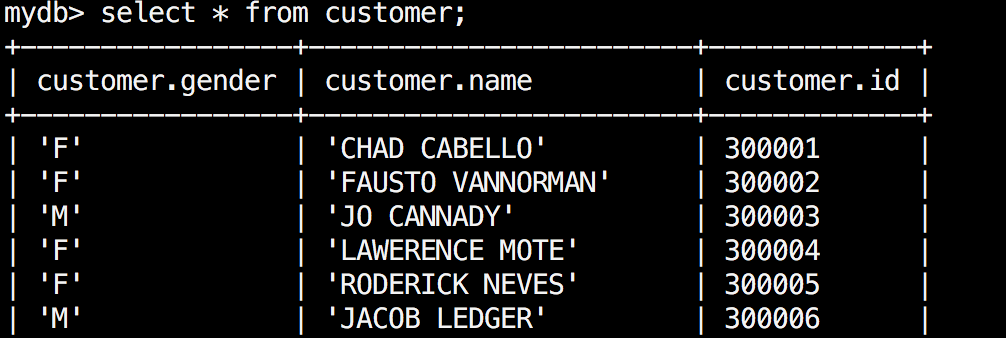
\includegraphics[width=11cm]{fig/mysql}
    \fcaption{\texttt{MySQL}风格打印}\label{myprint}
\end{center}

接下来我们列出\texttt{mydb}支持的SQL。

\subsubsection{\texttt{mydb}关键字}

\renewcommand{\t}[1]{\texttt{\textbf{#1}}}

\begin{center}
    (case not sensitive)
\begin{tabular}{llllll}
    \t{DATABASE} &\t{DATABASES} &\t{TABLE} &\t{TABLES} &\t{SHOW} &\t{CREATE} \\
    \t{DROP} &\t{USE} &\t{CHECK} &\t{PRIMARY} &\t{KEY} &\t{UNIQUE} \\
    \t{NOT} &\t{NULL} &\t{AUTO_INCREMENT} &\t{INSERT} &\t{INTO} &\t{VALUES} \\
    \t{DELETE} &\t{FROM} &\t{WHERE} &\t{UPDATE} &\t{SET} &\t{SELECT} \\
    \t{GROUP} &\t{BY} &\t{IS} &\t{IN} &\t{BETWEEN} &\t{LIKE} \\
    \t{AND} &\t{OR} &\t{SUM} &\t{AVG} &\t{MAX} &\t{MIN} \\
    \t{INT} &\t{SMALLINT} &\t{BIGINT} &\t{FLOAT} & \t{REAL} &\t{DOUBLE} \\
    \t{VARCHAR} &\t{STRING} &\t{CHAR} &\t{BOOLEAN} &\t{DATETIME} &\t{DESC}\\
    \t{FOREIGN} &\t{REFERENCES} & \t{INDEX} & \t{DEFAULT} & \t{TRUE} &\t{FALSE} \\
\end{tabular}
\end{center}


\subsubsection{\texttt{mydb}文法}

\renewcommand{\t}[1]{\texttt{\textbf{#1}}}

\setlength{\grammarindent}{10em}
\begin{grammar}

<program> ::= <stmt> [<stmt>]*

<ident> ::= \texttt{[A-Za-z_][A-Za-z0-9_]*}

<integer> ::= \texttt{(+|-)?[0-9]+}

<length> ::= \texttt{[0-9]+}

<real> ::= \texttt{(+|-)?[0-9]+.[0-9]+}

<string> ::= \texttt{'.*'}

<bool> ::= \t{TRUE} | \t{FALSE}

<value> ::= <integer> | <real> | <string> | <bool> | \t{NULL}

<stmt> ::= <sysStmt> \t{;}
\alt <dbStmt> \t{;}
\alt <tbStmt> \t{;}
\alt <idxStmt> \t{;}

<sysStmt> ::= \t{SHOW} \t{DATABASES}

<dbStmt> ::= \t{CREATE} \t{DATABASE} <dbName>
\alt \t{DROP} \t{DATABASE} <dbName>
\alt \t{USE} <dbName>
\alt \t{SHOW} \t{TABLES}

<tbStmt> ::= \t{CREATE} \t{TABLE} <tbName> \t{(} <field> [\t{,} <field>]* \t{)}
\alt \t{DROP} \t{TABLE} <tbName>
\alt \t{DESC} <tbName> | \t{SHOW} \t{TABLE} <tbName>
\alt \t{INSERT} \t{INTO} <tbName> [\t{(} <colName> [\t{,} <colName>]* \t{)}] \t{VALUES} \t{(} <values> \t{)} [\t{,} \t{(} <values> \t{)}]*
\alt \t{DELETE} \t{FROM} <tbName> \t{WHERE} <boolExpr>
\alt \t{UPDATE} <tbName> \t{SET} <colName> \t{=} <expr> [\t{,} <colName> \t{=} <expr>]* \t{WHERE} <boolExpr>
\alt \t{SELECT} <selectors> \t{FROM} <tbName> [\t{,} <tbName>]* [\t{WHERE} <boolExpr>] [\t{GROUP} \t{BY} <colName>]

<tbName> ::= <ident>

<colName> ::= <ident>

<field> ::= <colName> <type> [<attr>]*
\alt \t{CHECK} \t{(} <boolExpr> \t{)}
\alt \t{PRIMARY} \t{KEY} \t{(} <colName> \t{)}
\alt \t{FOREIGN} \t{KEY} \t{(} <colName> \t{)} \t{REFERENCES} <tbName> \t{(} <colName> \t{)} \t{)}

<type> ::= \t{INT} [\t{(} <length> \t{)}]
\alt \t{SMALLINT}
\alt \t{BIGINT}
\alt \t{FLOAT} | \t{REAL}
\alt \t{DOUBLE}
\alt \t{VARCHAR} \t{(} <length> \t{)}
\alt \t{STRING}
\alt \t{CHAR}
\alt \t{BOOLEAN}
\alt \t{DATETIME}

<attr> ::= \t{NOT} \t{NULL} | \t{UNIQUE} | \t{AUTO_INCREMENT} | \t{DEFAULT} <value>

<values> ::= <value> [\t{,} <value>]*

<boolExpr> ::= <col> <boolOp> <expr>
\alt <col> \t{IS} [\t{NOT}] \t{NULL}
\alt <col> [\t{NOT}] \t{IN} \t{(} <value> [\t{,} <value>]* \t{)}
\alt <col> [\t{NOT}] \t{BETWEEN} <value> \t{AND} <value>
\alt <col> [\t{NOT}] \t{LIKE} <string>
\alt \t{(} <boolExpr> \t{)}
\alt <boolExpr> \t{AND} <boolExpr>
\alt <boolExpr> \t{OR} <boolExpr>

<col> ::= [<tbName> \t{.}] <colName>

<boolOp> ::= `=' | `<>' | `<=' | `>=' | `<' | `>'

<expr> ::= <value>
\alt <col>
\alt <expr> <op> <expr>
\alt \t{(} <expr> \t{)}

<op> ::= `+' | `-' | `*' | `/' | `\%'

<selectors> ::= \t{*} | <selector> [\t{,} <selector>]*

<selector> ::= <col>
\alt <func> \t{(} <col> \t{)}

<func> ::= \t{SUM} | \t{AVG} | \t{MAX} | \t{MIN}

<idxStmt> ::= \t{CREATE} \t{INDEX} <tbName> \t{(} <colName> \t{)}
\alt \t{DROP} \t{INDEX} <tbName> \t{(} <colName> \t{)}

\end{grammar}


\subsubsection{\texttt{mydb}运算符优先级}

\renewcommand{\t}[1]{\texttt{\textbf{#1}}}

\begin{center}
    (from lowest to highest)\\
    \begin{tabular}{cl}
        left & \t{or} \\
        left & \t{and} \\
        left & \t{+} \t{-} \\
        left & \t{*} \t{/} \t{\%} \\
    \end{tabular}
\end{center}



\subsection{SQL执行模块}

在本模块中,我们将在数据库上实际执行上一模块解析出的SQL命令。

\begin{itemize}
\item 对于\texttt{USE, CREATE, DROP}等这种对表结构进行操作的命令,送往系统管理模块执行。
\item 对于\texttt{INSERT, UPDATE, DELETE, SELECT}等这种涉及记录的命令,将在本模块中通过调用系统管理模块和记录管理模块提供的功能来完成。
\end{itemize}

我们定义了一个\texttt{Evaluator}类,可以对包含列名的表达式求值。

下面我们将详细列举各命令、功能的实现原理及方法。

\subsubsection{\texttt{INSERT}}\label{sec:insert}

我们支持两种格式的\texttt{INSERT}。对于不指定列名的格式,我们根据创建表时给出的列顺序将表数据填入这条记录的相应位置,否则按照给出的列名填入。在填入用户给定的数据前,我们需要初始化\texttt{NULL}列的内容,以及在记录中填入默认值和自增字段的值。在填入数据时,我们会对列数据格式作兼容性检查。在填入数据后,我们会检查该记录是否满足所有的约束。最后,若一切条件均满足,便调用记录管理模块将该条记录写入数据库,同时更新有关索引。

\subsubsection{\texttt{SELECT}}\label{sec:select}

由于\texttt{SELECT}语句格式比较复杂,我们还支持聚集函数、\texttt{GROUP BY}和多表连接,因此在我们的实现中分四个步骤进行。

\begin{description}
\item[Query] 在此阶段,我们会根据\texttt{WHERE}子句的语法树生成一个filter函数对象,并将filter函数传入记录管理模块,在相应表的记录中将所有可能符合条件的记录找出。此处的可能是指在多表连接查询中,忽略了其余表的条件时的情况。这一阶段也就是\texttt{WHERE}子句的处理过程。
\item[Join] 在此阶段,我们会使用递归将上一阶段在所有表中查出的记录做笛卡尔积,同时再次应用filter函数找出所有符合条件的记录。
\item[Group By] 在此阶段,我们会根据\texttt{GROUP BY}子句将上一阶段得到的结果分组。若\texttt{GROUP BY}为空,则分为1组。
\item[Aggregate] 在此阶段,我们会对上一阶段中得到的所有组中的记录分别应用聚集函数,得到每组中的结果。若聚集函数为空,则返回所有结果。
\end{description}

经过以上四个步骤后,我们便得到了\texttt{SELECT}语句的结果,最后将其打印出来即可。

\subsubsection{\texttt{UPDATE}}

首先,我们会根据\texttt{WHERE}语句查出所有符合条件的需要更新的记录(查询的详细方法见\ref{sec:select})。在查出需要更新的记录后,由原记录计算\texttt{SET}子句中表达式的值,然后的处理流程与\ref{sec:insert} \texttt{INSERT}完全类似。

\subsubsection{\texttt{DELETE}}

对于\texttt{DELETE}命令,同样根据\texttt{WHERE}语句查出符合条件的记录,然后就可以调用记录管理模块删除这些记录以及对应的索引了。

\subsubsection{\texttt{USE, CREATE / DROP DATABASE / TABLE}}

对于这几个命令,直接调用系统管理模块完成相应功能。

注意对于\texttt{CREATE TABLE}命令,我们会增加一个隐藏的列NULL,以记录每列是否为空。

\subsubsection{\texttt{CREATE / DROP INDEX}}

对于建立、删除索引命令,由记录管理模块完成相应操作。

建立索引时,在记录管理模块中新建一个\texttt{multimap},并将所有记录的相应列值加入\texttt{multimap}中。

删除索引时,直接删除\texttt{multimap}。

\subsubsection{\texttt{CHECK}}

对于\texttt{CHECK}约束,在建表时将\texttt{BoolExpr}序列化保存下来,每当插入或更新记录时,对该表达式求值并判断真值即可。

\subsubsection{\texttt{PRIMARY KEY, FOREIGN KEY, UNIQUE, NOT NULL}}

\texttt{PRIMARY KEY}相当于\texttt{UNIQUE} + \texttt{NOT NULL}。

这四个约束在插入或更新记录时检查。

\begin{itemize}
\item 对于\texttt{NOT NULL},直接检查\texttt{NULL}列中对应位即可。
\item 对于\texttt{PRIMARY KEY}和\texttt{FOREIGN KEY},使用索引在记录管理模块中寻找该列是否存在相应的值。
\end{itemize}

\subsubsection{\texttt{WHERE}子句的扩展运算}

\begin{itemize}
\item 对于\texttt{BETWEEN}运算,我们只支持数值类型\texttt{BETWEEN},直接将其转化为\texttt{>=}和\texttt{<=}运算执行。
\item 对于\texttt{IN}运算,我们直接循环每个值,判断是否相等。
\item 对于\texttt{LIKE}运算,我们将查询字符串转换为正则表达式,然后调用正则表达式匹配。具体来说,将\texttt{\%}转换为\texttt{.*},将\texttt{\_}转换为\texttt{.},将\texttt{[!set]}中的\texttt{!}转换为\texttt{\^}。
\end{itemize}

\subsection{用户交互模块}

在顶层,我们设计了一个交互式终端,方便用户键入SQL语句并执行数据库操作。输入\texttt{exit}或\texttt{quit}可以退出终端。我们还支持多行输入SQL语句  (如\fref{inter:multi}),以\texttt{;}作为语句的结束。

\begin{center}
    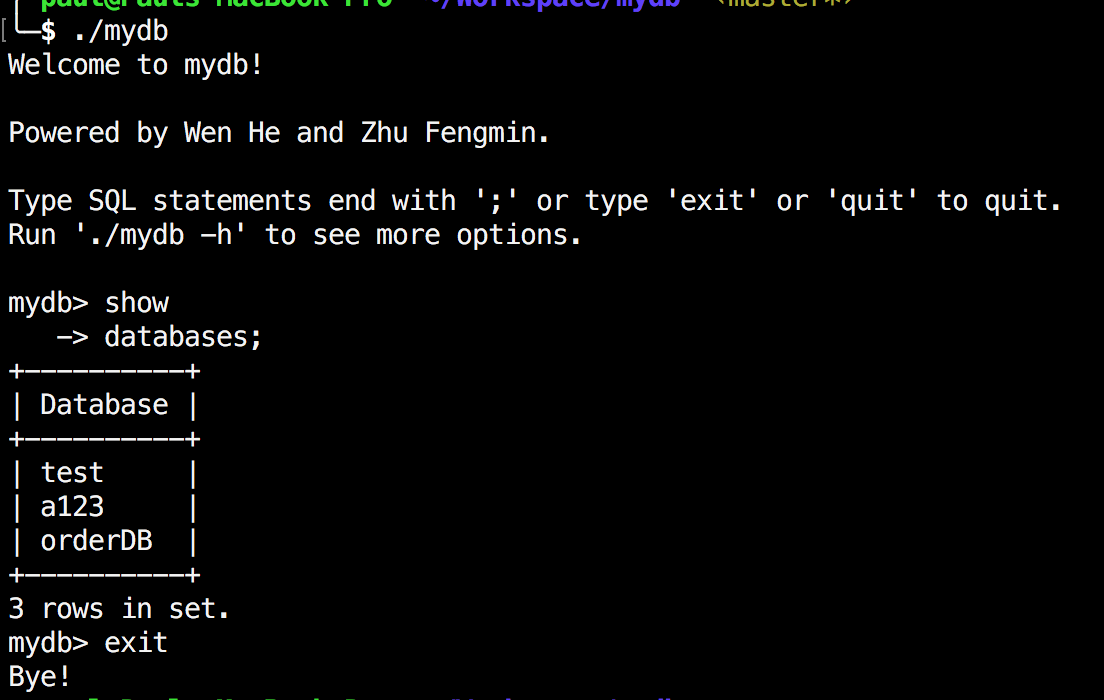
\includegraphics[width=11cm]{fig/multi-row}
    \fcaption{交互式终端允许多行输入}\label{inter:multi}
\end{center}

此外,我们还利用Linux的\texttt{socket} API实现了远程数据库连接。具体来说,就是通过\texttt{socket} 把客户端的SQL语句发送给服务端,服务端接收到命令后调用SQL解析模块,操作完成后,将返回的结果字符串通过\texttt{socket}回送给客户端,客户端将其显示出来。

\section{测试结果}

接下来我们对\texttt{mydb}实现的功能一一进行测试。

\subsection{数据库管理及查询功能}

首先,我们打开\texttt{mydb},新建一个数据库\texttt{test}并切换到它。

\begin{center}
    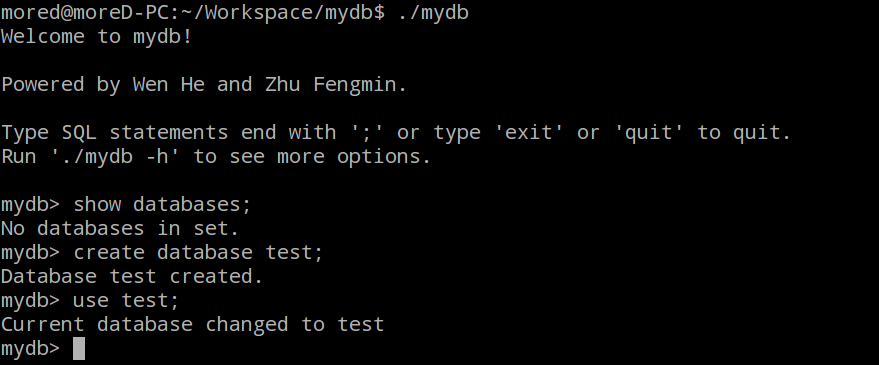
\includegraphics[width=12cm]{fig/create-db}
    \fcaption{新建数据库并切换}
\end{center}

然后,我们新建一个带有主键、自增字段、默认值字段的表,再新建一个有唯一字段、非空字段、域完整性约束和外键的表。建立表结构后,我们往表里添加一些合法记录。

\begin{center}
    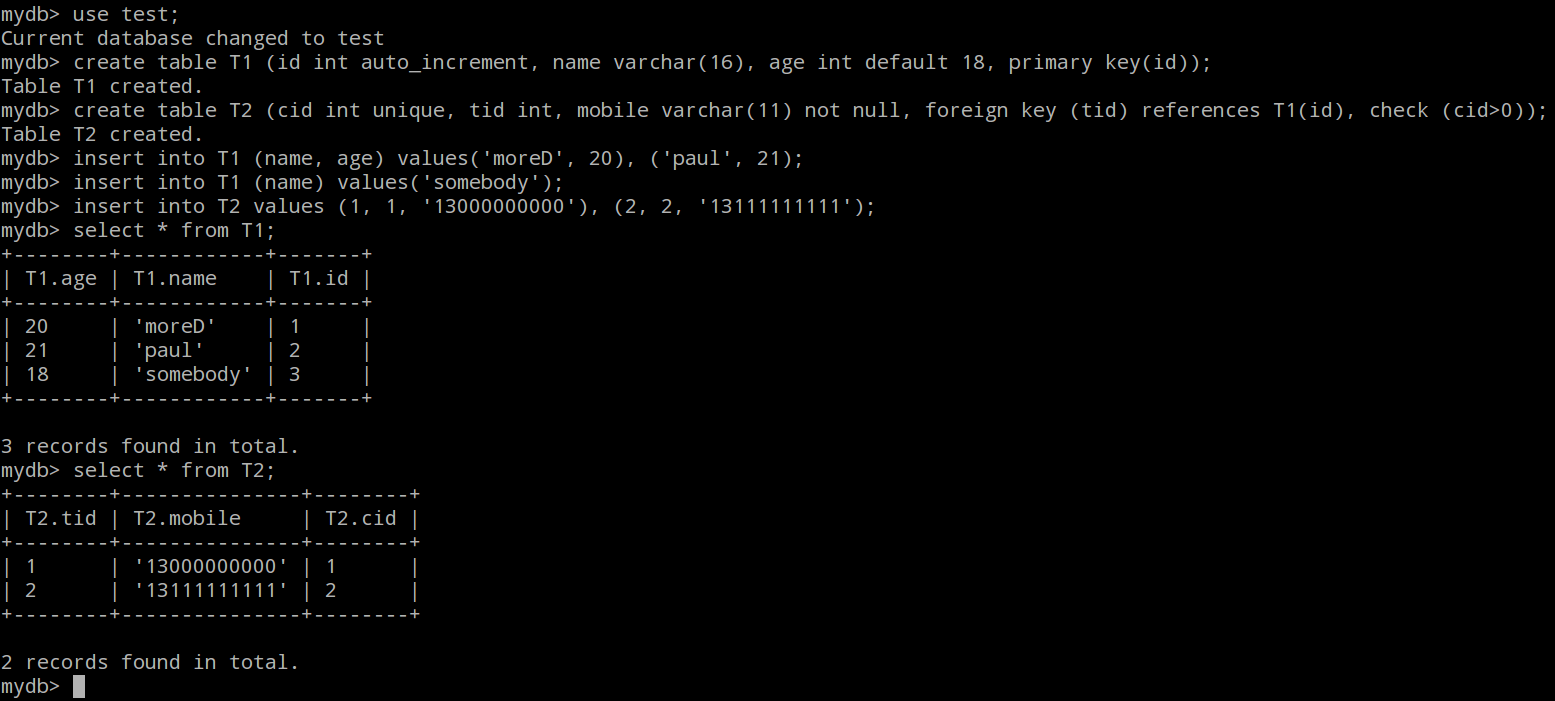
\includegraphics[width=15cm]{fig/create-table}
    \fcaption{建表并插入记录}
\end{center}

我们再尝试往表里添加非法记录。

\begin{center}
    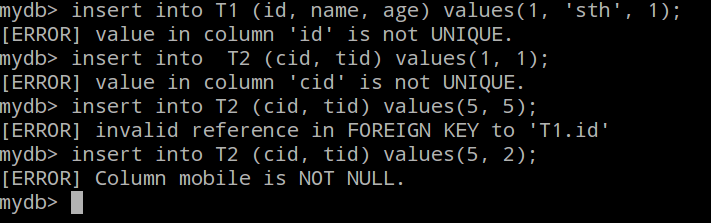
\includegraphics[width=10cm]{fig/illegal-record}
    \fcaption{插入非法记录时报错}
\end{center}

然后我们尝试使用各种查询语句。

\begin{center}
    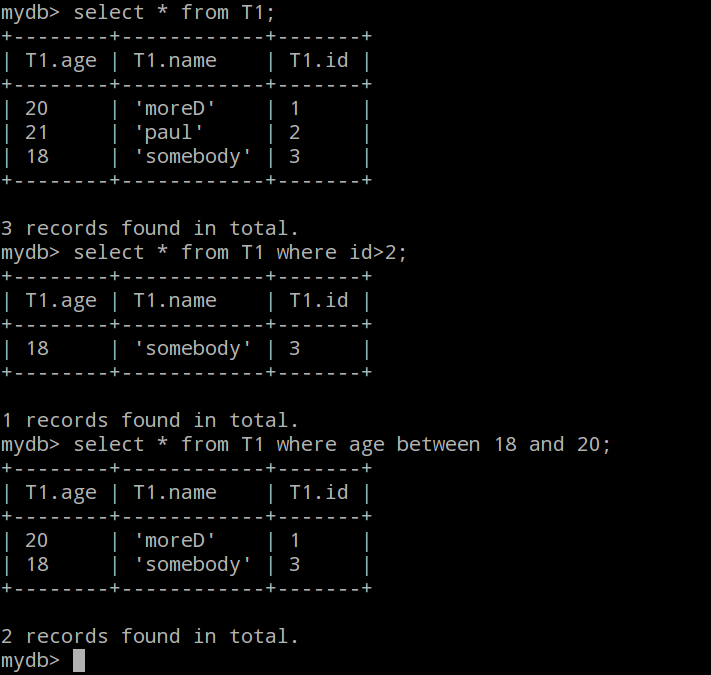
\includegraphics[width=9cm]{fig/query1}
    \fcaption{查询1}
\end{center}

\begin{center}
    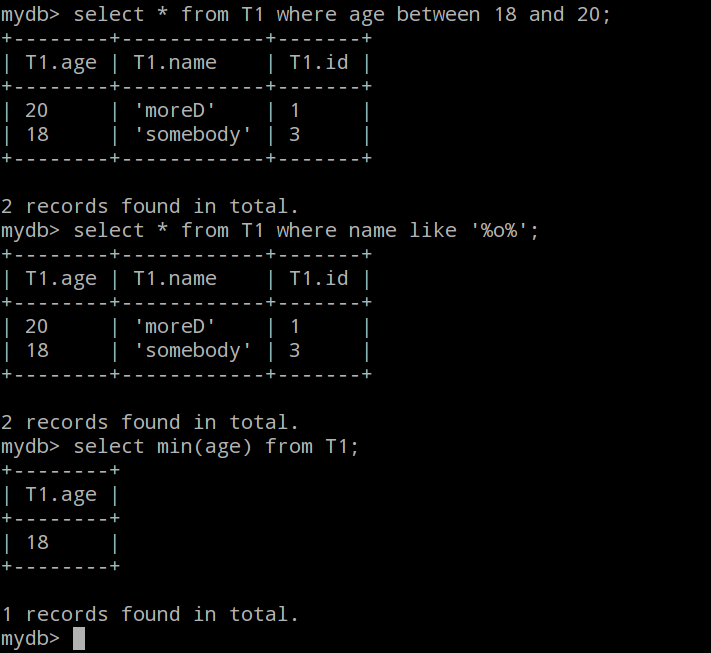
\includegraphics[width=9cm]{fig/query2}
    \fcaption{查询2}
\end{center}

\begin{center}
    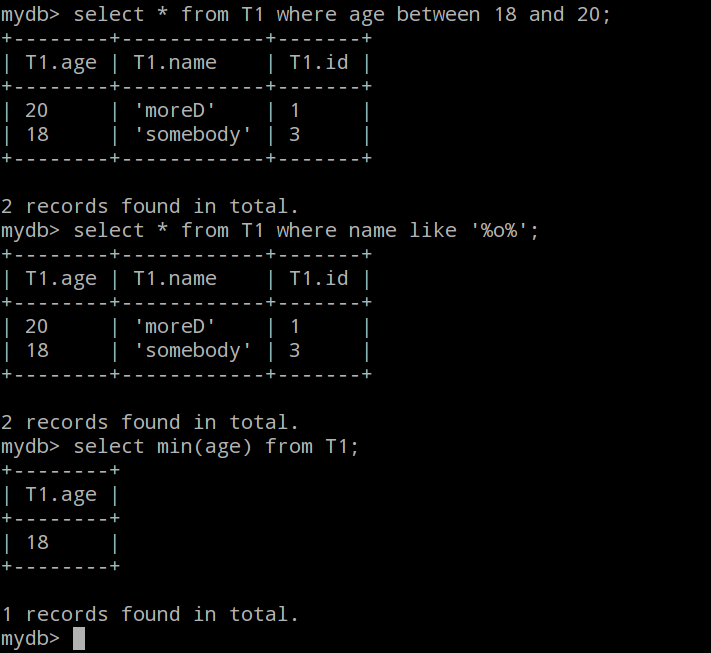
\includegraphics[width=9cm]{fig/query2}
    \fcaption{查询3}
\end{center}

再尝试更新和删除语句。

\begin{center}
    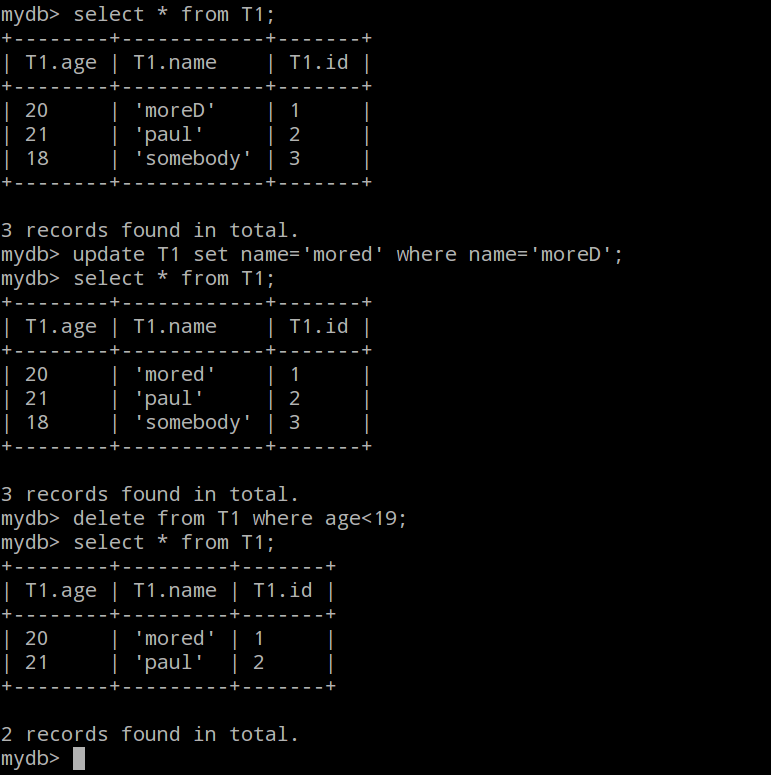
\includegraphics[width=10cm]{fig/update-delete}
    \fcaption{更新和删除}
\end{center}

最后删除表和数据库。

\begin{center}
    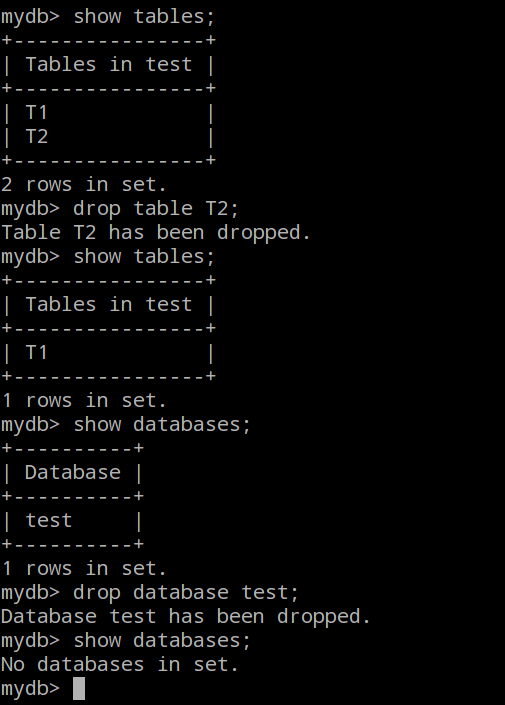
\includegraphics[width=8cm]{fig/drop-db}
    \fcaption{删除表及数据库}
\end{center}

\subsection{远程连接功能}

首先,我们启动一个服务端。

\begin{center}
    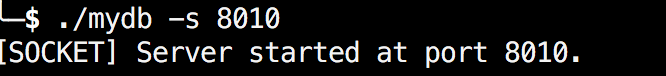
\includegraphics[width=8cm]{fig/server}
    \fcaption{启动服务端}
\end{center}

接下来,我们通过客户端连接服务端。

\begin{center}
    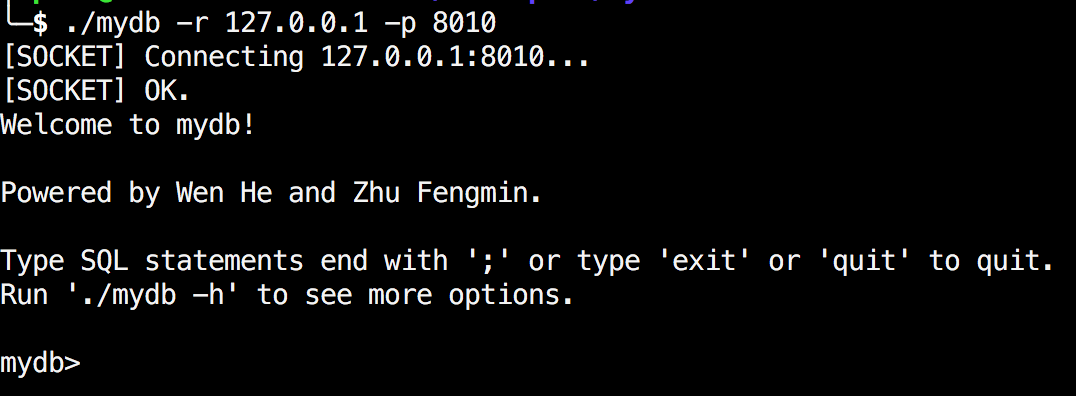
\includegraphics[width=11cm]{fig/conn}
    \fcaption{客户端连接服务端}
\end{center}

最后,我们输入一系列SQL语句,测试服务端返回的信息都是正确的。

\begin{center}
    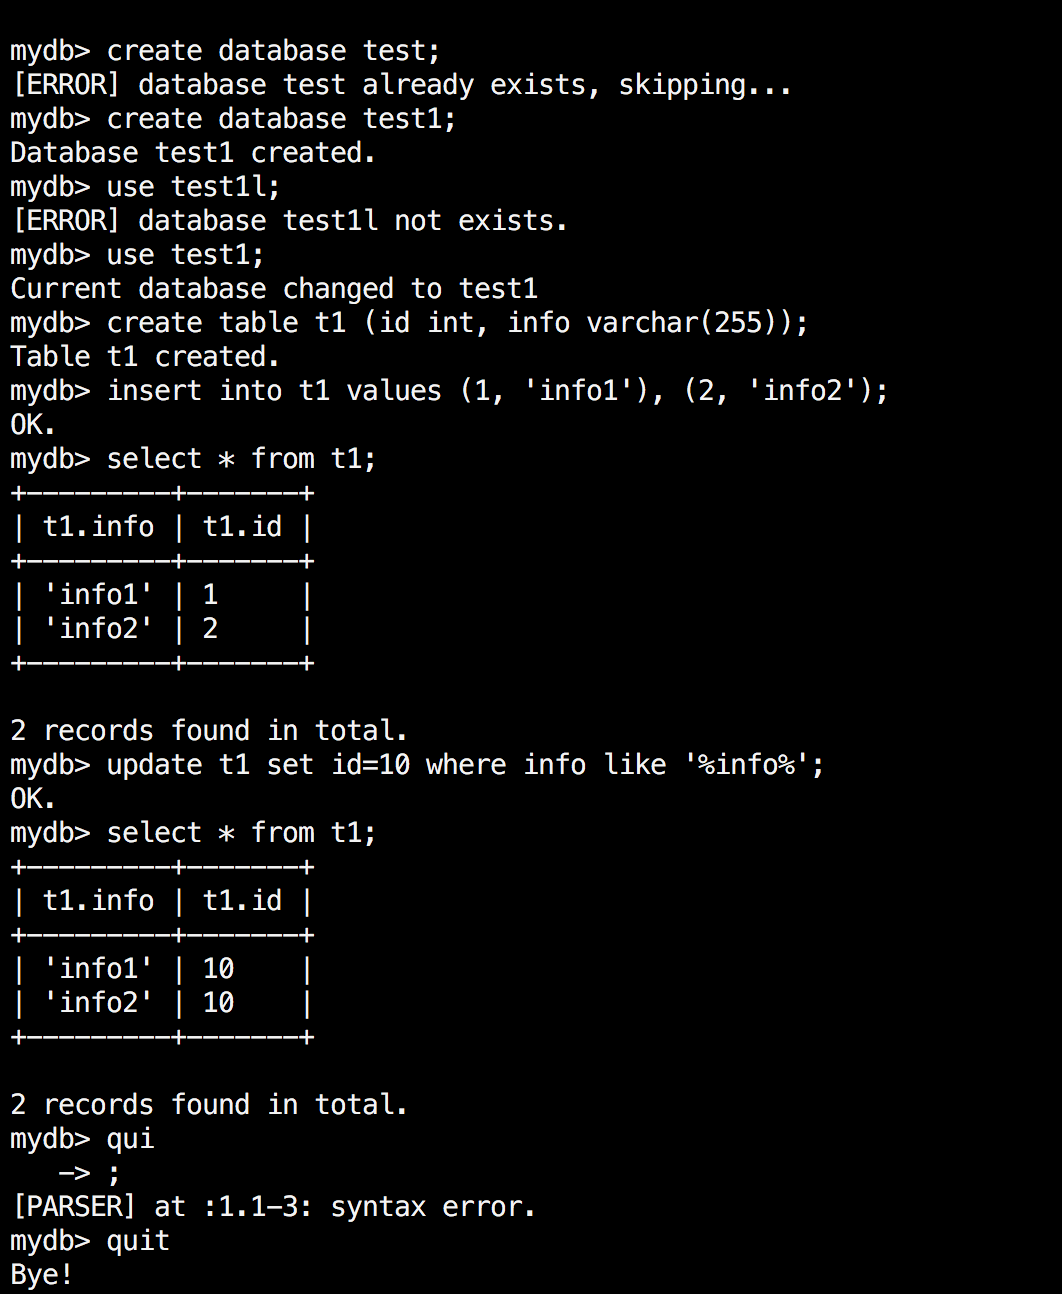
\includegraphics[width=11cm]{fig/conn-test}
    \fcaption{远程操作数据库}
\end{center}

退出客户端后,服务端仍然等待新的客户端连接。

\begin{center}
    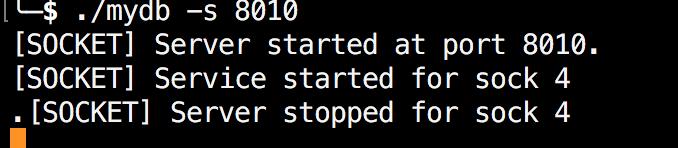
\includegraphics[width=8cm]{fig/disconn}
    \fcaption{断开连接}
\end{center}

\section{项目链接}

\url{https://github.com/paulzfm/mydb}

\section{使用方法}

详见\texttt{README.md},或前往Github:\url{https://github.com/paulzfm/mydb#mydb}。

\section{小组分工}

请见\tref{jobs}。

\begin{center}
    \tcaption{小组分工}\label{jobs}
    \begin{tabular}{ll}
        \toprule
        功能 & 负责人 \\
        \midrule
        记录管理 & 朱俸民 \\
        系统管理 & 温和 \\
        SQL解析与语义检查 & 朱俸民 \\
        查询执行 & 温和 \\
        交互终端与远程连接 & 朱俸民 \\
        索引 & 温和 \\
        \bottomrule
    \end{tabular}
\end{center}

\renewcommand{\refname}{参考资料}

\begin{thebibliography}{9}

\bibitem{bib1} Bison. \url{https://engineering.purdue.edu/~milind/ece573/2015fall/project/bison.html}.

\bibitem{bib2} SQL Tutorial. \url{http://www.w3schools.com/sql/default.asp}.

\bibitem{bib3} 冯建华, 周立柱. 数据库系统设计与原理. 

\bibitem{bib4} cppreference. \url{http://en.cppreference.com/}.

\bibitem{bib5} RapidJSON. \url{http://rapidjson.org/index.html}.

\end{thebibliography}

\end{document}
